\section{Manuel d'utilisation}
manuel d'utilisation pour artiste (léger, avec i-score create device) et pour développeur () 

\section{Chorégraphie}
Voici la chorégraphie sous forme de storyboard conçue par les étudiants d'Art de l'université de Bilbao. On peut distinguer que le spectacle est divisé en plusieurs parties, l'image du storyboard correspondant est indiqué entre parenthèses : le réveil (1), la rencontre (2), la danse (3-10), la percussion avec un rythme particulier engendré par les pattes des robots (11-12), la dernière ronde (13), le retrait (14-18).

\hspace*{-2cm}
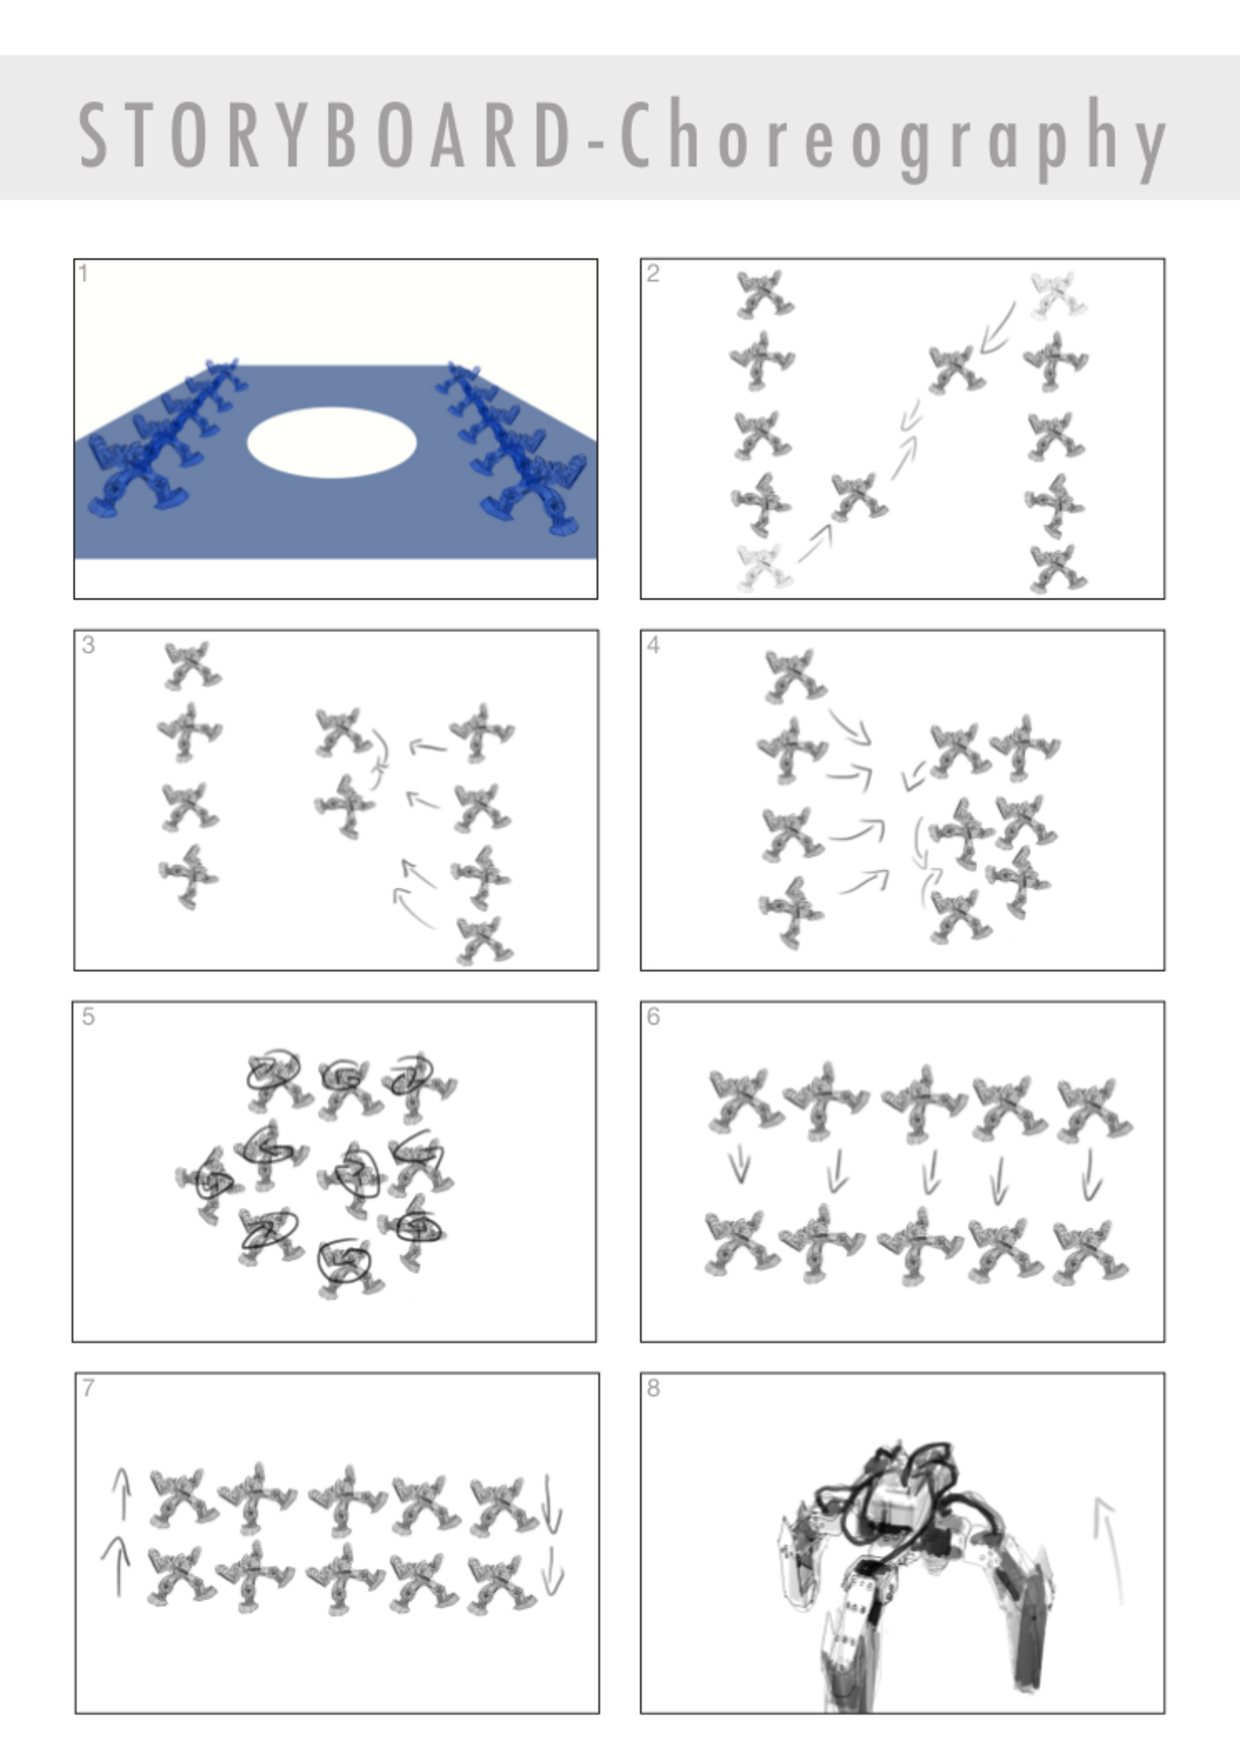
\includepdf[pages={1,2},scale=0.9]{storyboard}
